%%%%%%%%%%%%%%%%%%%%%%%%%%%%%%%%%%%%%%%%%
% Journal Article
% LaTeX Template
% Version 1.4 (15/5/16)
%
% This template has been downloaded from:
% http://www.LaTeXTemplates.com
%
% Original author:
% Frits Wenneker (http://www.howtotex.com) with extensive modifications by
% Vel (vel@LaTeXTemplates.com)
%
% License:
% CC BY-NC-SA 3.0 (http://creativecommons.org/licenses/by-nc-sa/3.0/)
%
%%%%%%%%%%%%%%%%%%%%%%%%%%%%%%%%%%%%%%%%%

%----------------------------------------------------------------------------------------
%	PACKAGES AND OTHER DOCUMENT CONFIGURATIONS
%----------------------------------------------------------------------------------------

\documentclass[twoside,twocolumn]{article}



\usepackage{blindtext} % Package to generate dummy text throughout this template 

\usepackage[sc]{mathpazo} % Use the Palatino font
\usepackage[T1]{fontenc} % Use 8-bit encoding that has 256 glyphs
\linespread{1.05} % Line spacing - Palatino needs more space between lines
\usepackage{microtype} % Slightly tweak font spacing for aesthetics

\usepackage[english]{babel} % Language hyphenation and typographical rules

\usepackage[hmarginratio=1:1,top=32mm,columnsep=20pt]{geometry} % Document margins
\usepackage[hang, small,labelfont=bf,up,textfont=it,up,figurename=Obrázek,tablename=Tabulka]{caption} % Custom captions under/above floats in tables or figures
\usepackage{booktabs} % Horizontal rules in tables

\usepackage{lettrine} % The lettrine is the first enlarged letter at the beginning of the text

\usepackage{enumitem} % Customized lists
\setlist[itemize]{noitemsep} % Make itemize lists more compact

\usepackage{abstract} % Allows abstract customization
\renewcommand{\abstractnamefont}{\normalfont\bfseries} % Set the "Abstract" text to bold
\renewcommand{\abstracttextfont}{\normalfont\small\itshape} % Set the abstract itself to small italic text

\usepackage{titlesec} % Allows customization of titles
\renewcommand\thesection{\Roman{section}} % Roman numerals for the sections
\renewcommand\thesubsection{\roman{subsection}} % roman numerals for subsections
\titleformat{\section}[block]{\large\scshape\centering}{\thesection.}{1em}{} % Change the look of the section titles
\titleformat{\subsection}[block]{\large}{\thesubsection.}{1em}{} % Change the look of the section titles

%\usepackage{fancyhdr} % Headers and footers
%\pagestyle{fancy} % All pages have headers and footers
%\fancyhead{} % Blank out the default header
%\fancyfoot{} % Blank out the default footer
%\fancyhead[C]{} % Custom header text
%\fancyfoot[RO,LE]{\thepage} % Custom footer text

\usepackage{titling} % Customizing the title section

\usepackage{hyperref}
\usepackage{graphicx} % For hyperlinks in the PDF


%----------------------------------------------------------------------------------------
%	TITLE SECTION
%----------------------------------------------------------------------------------------

\setlength{\droptitle}{-4\baselineskip} % Move the title up

\pretitle{\begin{center}\Huge\bfseries} % Article title formatting
\posttitle{\end{center}} % Article title closing formatting
\title{Heuristika simulovaného ochlazování pro řešení MaxWeightedSAT} % Article title
\author{%
    \textsc{Luboš Zápotočný}\\[1ex] % Your name
    \normalsize České vysoké učení technické v Praze - fakulta informačních technologií \\ % Your institution
    \normalsize \href{mailto:zapotlub@fit.cvut.cz}{zapotlub@fit.cvut.cz} % Your email address
%\and % Uncomment if 2 authors are required, duplicate these 4 lines if more
%\textsc{Jane Smith}\thanks{Corresponding author} \\[1ex] % Second author's name
%\normalsize University of Utah \\ % Second author's institution
%\normalsize \href{mailto:jane@smith.com}{jane@smith.com} % Second author's email address
}
\date{} % Leave empty to omit a date \today
%\renewcommand{\maketitlehookd}{%
%\begin{abstract}
%\noindent \blindtext % Dummy abstract text - replace \blindtext with your abstract text
%\end{abstract}
%}

%----------------------------------------------------------------------------------------

\begin{document}

% Print the title
    \maketitle

%----------------------------------------------------------------------------------------
%	ARTICLE CONTENTS
%----------------------------------------------------------------------------------------


    \section{Úvod}

    Problém splnitelnosti booleovské formule (ozačováno z angličtiny SATISFIABILITY, zkráceně SAT) označuje problém
    nalezení splňujícího (vyhovujícího) ohodnocení logické formule v~konjunktivní normálním formě tak, aby byly všechny její
    klauzule splněné.

    SAT byl první problém o kterém se dokázalo, že je NP-úplný~\cite{CookLevin1971}.
    Tedy pro tento problém neexistuje (za předpokladu P $\neq$ NP) efektivní algoritmus, který by tento problém řešil v polynomiálním čase.
    Jelikož se jedná o NP-těžký (NP-úplné problémy jsou podmnožinou NP-těžkých) problém, lze na tento problém převést instance všech problému ze tříd P a NP.

    MaxWeightedSAT označuje optimalizační verzi hledání SAT ohodnocení zároveň s kritériem pro maximalizace součtu
    vah proměnných ohodnocených 1 (True).
    Problém je tedy rozšířen o atributy $w(x_i)$ pro všechny proměnné $w_i$ reprezentující váhové ohodnocení jednotlivých
    proměnných.

    Tato práce se zaměřuje na řešení výše zmíněného NP-těžkého optimzačního problému pomocí heuristiky simulovaného ochlazování.

    Algoritmus náhodně prochází stavovým prostorem ohodnocení proměnných formule tak, aby maximalizoval součet vah pozitivně
    ohodnocených proměnných a zároveň aby toto ohodnocení splňovanou zadanou formuli.

    Stavový prostor je tedy vektor (pole) boolevských ohodnocení (True/False) jednotlivých proměnných.
    Operátorem přechodu do nového stavu je logická změna jednoho náhodného bitu v tomto vektoru.

    Algoritmus přechází do zlepšíjících stavů a s určitou pravděpodobností přechází také do zhrošujících stavů.
    Tímto postupem se heuristika snaží zamezit uvízní v lokálních extrémech.

    Heuristika začíná s vysokou teplotou, která ovlivňuje mimo jiné také pravděpodobnost přijetí nezlepšujících stavů.
    To vede k velkému prozkoumání stavového prostoru v prvních krocích algoirtmu.
    Každý krok algorimu sníží tuto teplotu o násobek chladícího faktoru (lineárně).
    Tímto chlazením se také snižuje pravděpodobnost přijetí zhrošujícího stavu a heuristika tímto konverguje k nalezení
    optimálního řešení.

%------------------------------------------------


    \section{Implementace}

    Heuristika a experimentální vyhodnocení byly naprogramovány v jazyce Python.
    Při hledání ideálních parametrů heuristiky či efektivity algoritmu není uvažována efektivita jazyka jako takového.
    Všechny metriky jsou univerzálně přenositelné mezi různými hardwarovými platformami.

    Hlavní část heuristiky je zobrazen na obrázku~\ref{fig:main-part} kde je vi

    \begin{figure}
        \centering
        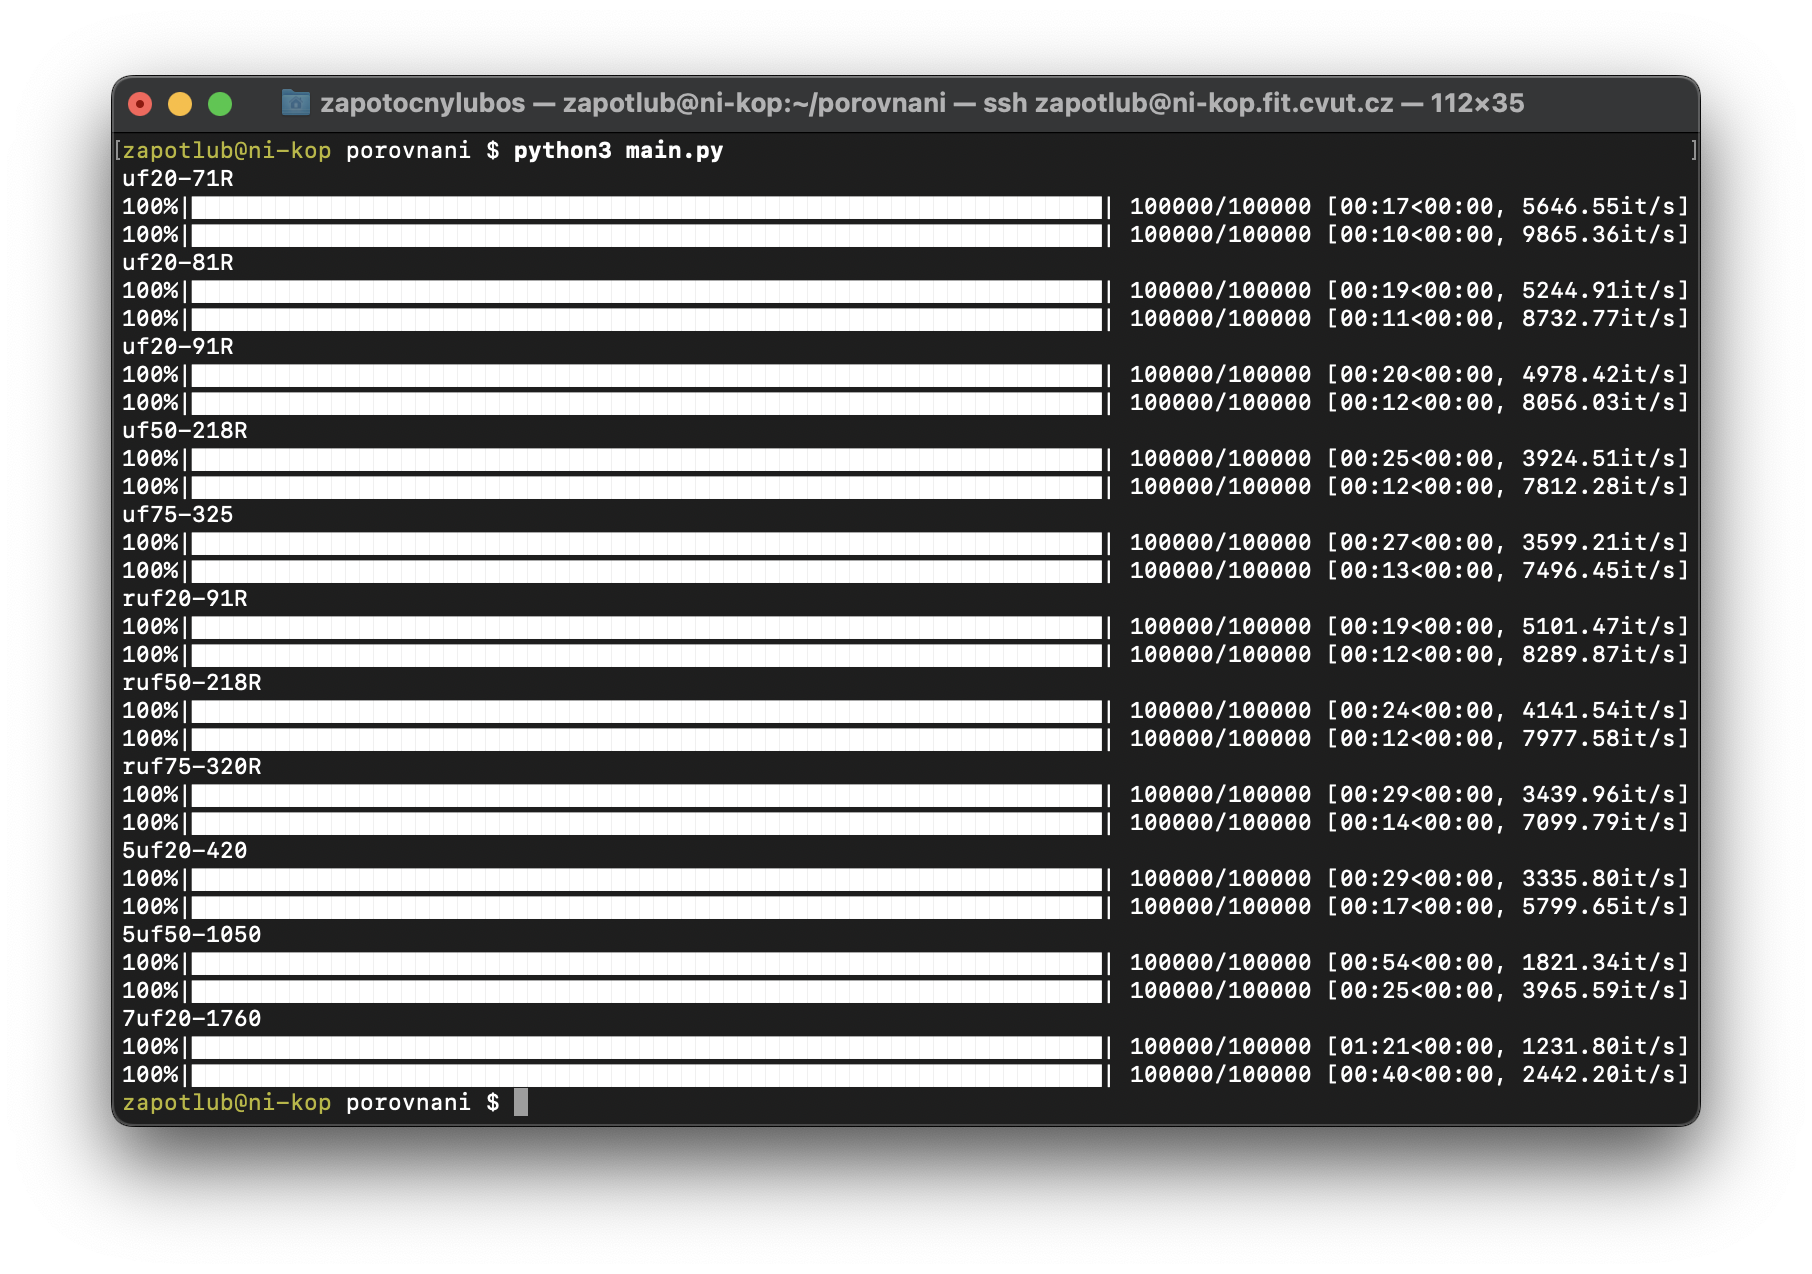
\includegraphics[width=7cm]{images/generation}
        \caption{Spuštění experimentu}
        \label{fig:main-part}
    \end{figure}

    V rámci experimentálního vyhodnocení úspěšnosti jednotlivých algoritmů byly algoritmy omezené na 500 možností převrácení hodnoty proměnné (flip).
    Efektivita algoritmů byla testována na splnitelných instancích SAT formulí ze sad

    \begin{itemize}
        \item uf20-71R
        \item uf20-81R
        \item uf20-91R
        \item uf50-218R
        \item uf75-325
        \item ruf20-91R
        \item ruf50-218R
        \item ruf75-320R
        \item 5uf20-420
        \item 5uf50-1050
        \item 7uf20-1760
    \end{itemize}

    Podrobný popis datových sad lze najít na stránkách kurzu NI-KOP~ČVUT~FIT~\cite{coursesData}

    Každá instance problému z datové sady byla spuštěna 1000 pro daný algoritmus, ale vždy s~jiným seedem pro pseudo náhodný generátor.
    Ve výsledku byl každý algoritmus otestován na 100000 spuštěních pro každou datovou sadu.
    Celkově se tedy pro získání experimentálních dat spustilo 2.2 milionu běhů algoritmu pro hledání splnitelného ohodnocení.

    \begin{figure}
        \centering
        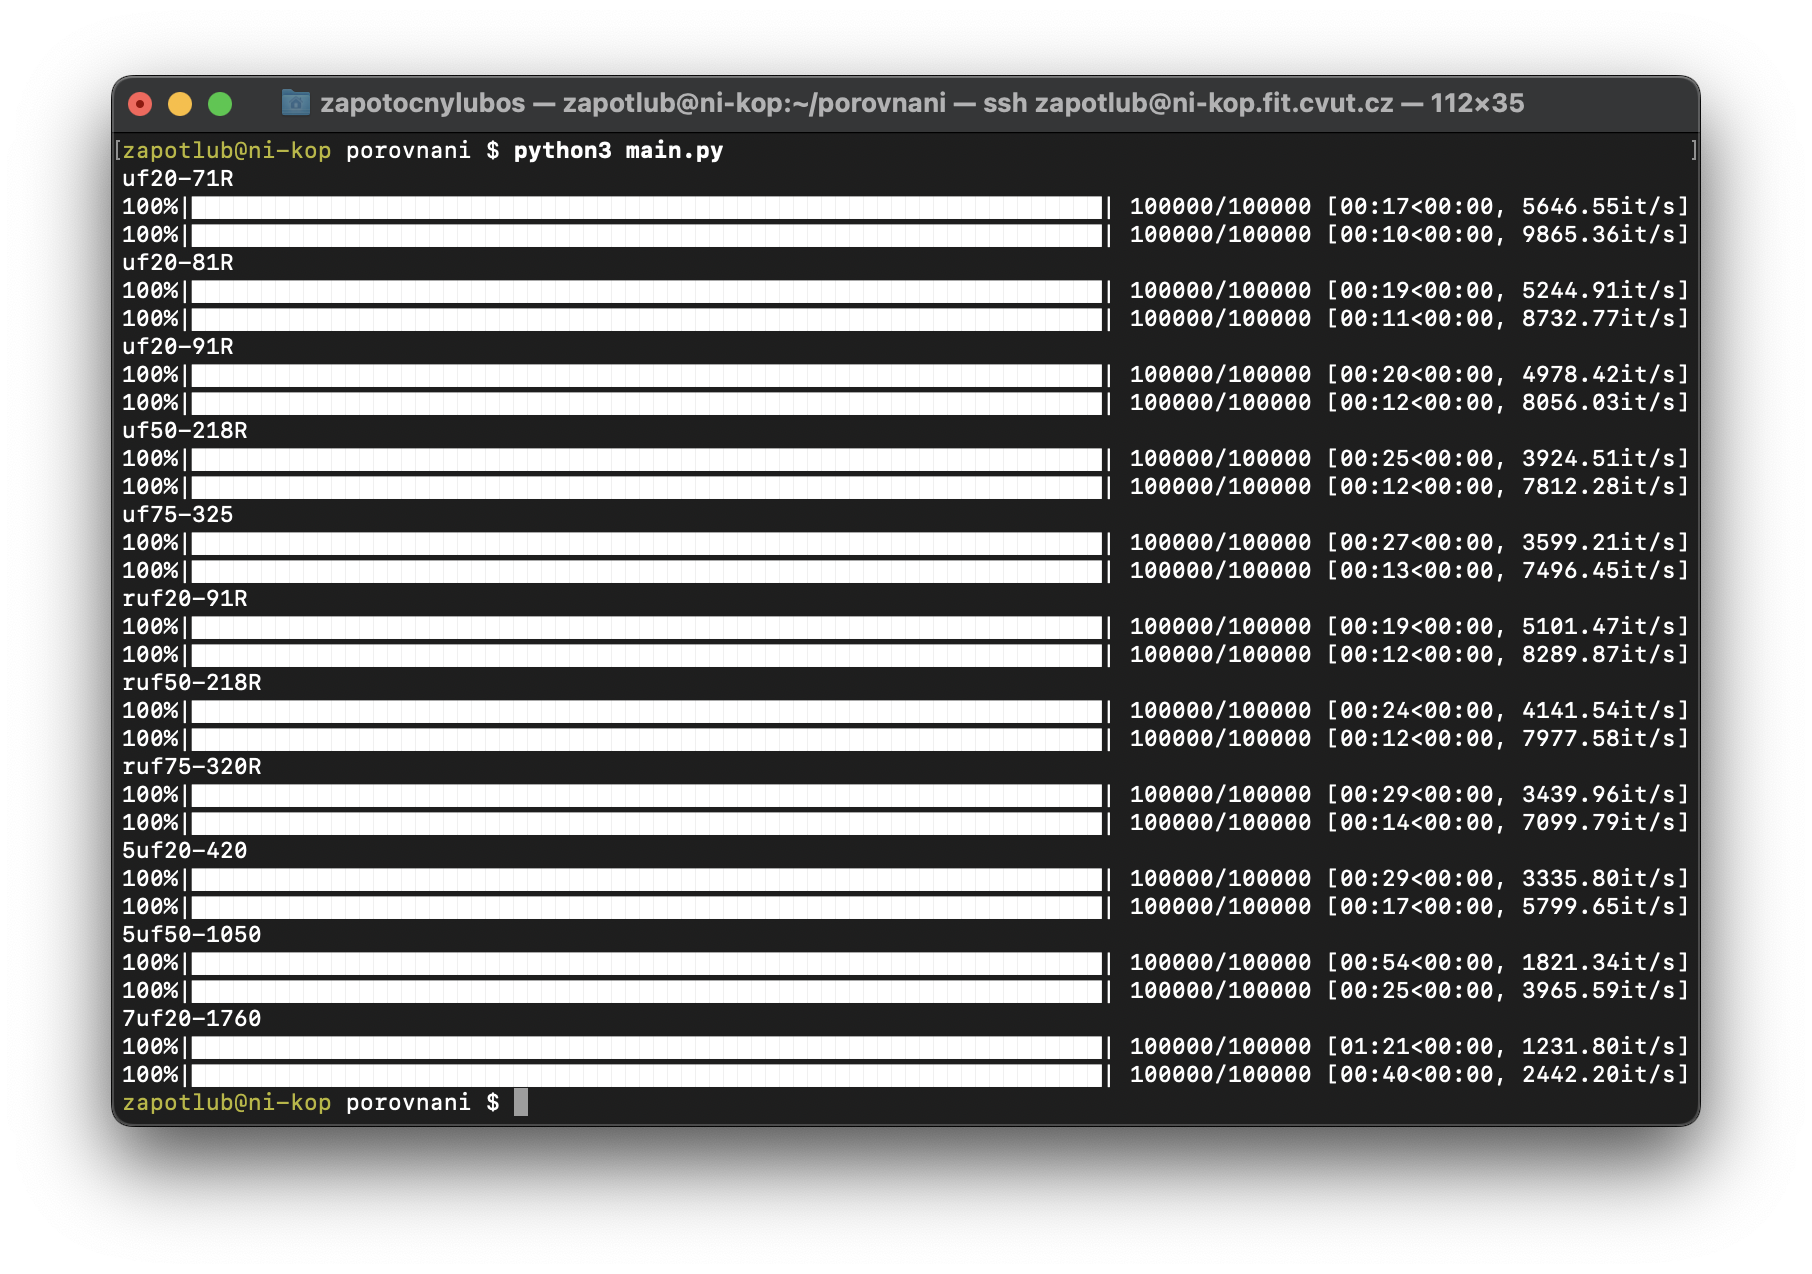
\includegraphics[width=7cm]{images/generation}
        \caption{Spuštění experimentu}
        \label{fig:generation}
    \end{figure}

    Obrázek~\ref{fig:generation} zobrazuje dokočení sběru experimentálních dat na datových sadách pro algortmus gSAT (první řádek)
    a také probSAT (druhý řádek).

    Algoritmy následně byly porovnány na základě úspěšnosti, tedy zdali daný alogoritmus dokázal vygenerovat
    splňující ohodnocení (splnitelné formule), a také na základě počtu iterací, než dané řešení dokázaly vygenerovat.

    Zkoumán byl také poměr úspěšných a~neúspěšných běhů algoritmu a také prúměrný počet iterací nutný k zastavení programu.
    Dále byl zkoumán průměrný počet iterací algoritmu pomocí váženého průměru,
    kde neúspěšné běhy byly penalizovány maximálním počtem iterací v dané datové sadě.
    Algorimy byly omezené na 500 iterací (flipů).

    Následně byla zkoumána distribuční funkce počtu iterací v úspěšných bězích algoritmu a~vzájemné křížení
    těchto distribučních funkcí mezi dvěma algoritmy.
    Také byla zkoumána korigovaná distribuční funkce, která zohledňuje neúspešné běhy algoritmu.

    Nakonec bylo zkoumáno, zdali se počet iterací úspěšných běhů řídí log-normálním statistickým rozložením.

%------------------------------------------------


    \section{Výsledky}


    Tabulka~\ref{tab:success_ratio} zobrazuje procentuální úspěšnost jednotlivých algoritmů na instancích z příslušné datové sady.
    Lze nahlédnout, že algoritmus probSAT byl na všech sadách úspěšnější (dokázal nalézt splnitelné ohodnocení proměnných).
    Algoritmus probSAT průměrně nalezl splňujicí ohodnocení v $66.2\%$ případech, kdežto gSAT pouze v $59.2\%$, jedná se tedy o $7\%$ rozdíl.


    \begin{table}
        \caption{Úspěšnost běhů}
        \centering
        \begin{tabular}{llr}
            \toprule
            Datová sada & gSAT     & probSAT  \\
            \midrule
            uf20-71R    & $100\%$  & $100\%$  \\
            uf20-81R    & $99.9\%$ & $100\%$  \\
            uf20-91R    & $94.1\%$ & $98.2\%$ \\
            uf50-218R   & $49.7\%$ & $63.7\%$ \\
            uf75-325    & $27.4\%$ & $38.7\%$ \\
            ruf20-91R   & $94.0\%$ & $97.8\%$ \\
            ruf50-218R  & $51.7\%$ & $64.6\%$ \\
            ruf75-320R  & $30.0\%$ & $42.5\%$ \\
            5uf20-420   & $67.7\%$ & $79.5\%$ \\
            5uf50-1050  & $4.6\%$  & $5.4\%$  \\
            7uf20-1760  & $31.7\%$ & $37.6\%$ \\
            \midrule
            Průměr      & $59.2\%$ & $66.2\%$ \\
            \bottomrule
        \end{tabular}
        \label{tab:success_ratio}
    \end{table}

    Tabulka~\ref{tab:average_iterations} zobrazuje průměrný počet iterací, které algoitmus provedl, než našel splňující
    ohodnocení nebo byl po 500 iteracích zastaven a danou formuli nedokázal splnit.
    Lze také pozorovat trend, že algoritmus probSAT potřeboval průměrně méně iterací pro nalezení řešení než gSAT\@.
    Algoritmus gSAT potřeboval průměrně $270$ iteraci, než nalezl splňující ohodnocení, kdežto probSAT potřeboval pouze $245.6$.
    ProbSAT tedy potřeboval v průměru o~$24.4$ iterací méně, než gSAT\@.


    \begin{table}
        \caption{Průměrný počet iterací}
        \centering
        \begin{tabular}{llr}
            \toprule
            Datová sada & gSAT    & probSAT \\
            \midrule
            uf20-71R    & $8.0$   & $8.0$   \\
            uf20-81R    & $13.1$  & $12.2$  \\
            uf20-91R    & $104.1$ & $76.9$  \\
            uf50-218R   & $346.0$ & $306.7$ \\
            uf75-325    & $429.6$ & $404.2$ \\
            ruf20-91R   & $106.4$ & $81.1$  \\
            ruf50-218R  & $337.4$ & $299.6$ \\
            ruf75-320R  & $423.3$ & $393.8$ \\
            5uf20-420   & $277.8$ & $233.7$ \\
            5uf50-1050  & $489.3$ & $488.9$ \\
            7uf20-1760  & $412.6$ & $396.5$ \\
            \midrule
            Průměr      & $270.0$ & $245.6$ \\
            \bottomrule
        \end{tabular}
        \label{tab:average_iterations}
    \end{table}

    Tabulka~\ref{tab:average_fined_iterations} zobrazuje vážený průměrný počet itarcí algoritmu na instancích z datových sad.
    Vážený průměr je zde počítán pomocí penalizace neúspěšných běhů alogitmu.
    Za předpokladu, že alogitmus nalezl splňující ohodnocení, do průměru se připočítá pouze počet iterací při daném běhu.
    Pokud ale algoritmus nedokázal nalézt splňující ohodnocení, do průměru se započítává počet iterací algoritmu společně s penalizací,
    která činí maximální počet iterací algoritmu přes všechny běhy nad instancemi z~dané datové sady.

    \begin{table}
        \caption{Vážený průměrný počet iterací}
        \centering
        \begin{tabular}{llr}
            \toprule
            Datová sada & gSAT    & probSAT \\
            \midrule
            uf20-71R    & $8.0$   & $8.0$   \\
            uf20-81R    & $13.1$  & $12.2$  \\
            uf20-91R    & $133.7$ & $85.9$  \\
            uf50-218R   & $597.4$ & $488.3$ \\
            uf75-325    & $792.4$ & $710.8$ \\
            ruf20-91R   & $136.4$ & $92.2$  \\
            ruf50-218R  & $578.9$ & $476.9$ \\
            ruf75-320R  & $774.7$ & $681.2$ \\
            5uf20-420   & $439.4$ & $336.0$ \\
            5uf50-1050  & $966.4$ & $962.1$ \\
            7uf20-1760  & $754.1$ & $708.3$ \\
            \midrule
            Průměr      & $472.3$ & $414.7$ \\
            \bottomrule
        \end{tabular}
        \label{tab:average_fined_iterations}
    \end{table}

    Dále v rámci experimentálního porovnání byla zkoumána distribuční funkce (její odhad) počtu kroků (iterací) algoritmů.
    Obrázek~\ref{fig:cdf1} a obrázek~\ref{fig:cdf2} znázorňují pravděpodobnosti, že daný algoritmus skončí do X kroků (${P[x <= X]}$).
    Distribuční funkce byla počítána pouze z úspešných běhů obou algoritmů.

    Algoritmus probSAT zvítězil v $7$ z $11$ datových sad.
    Algoritmus gSAT pouze v $4$ z $11$.

    \begin{figure*}[h]
        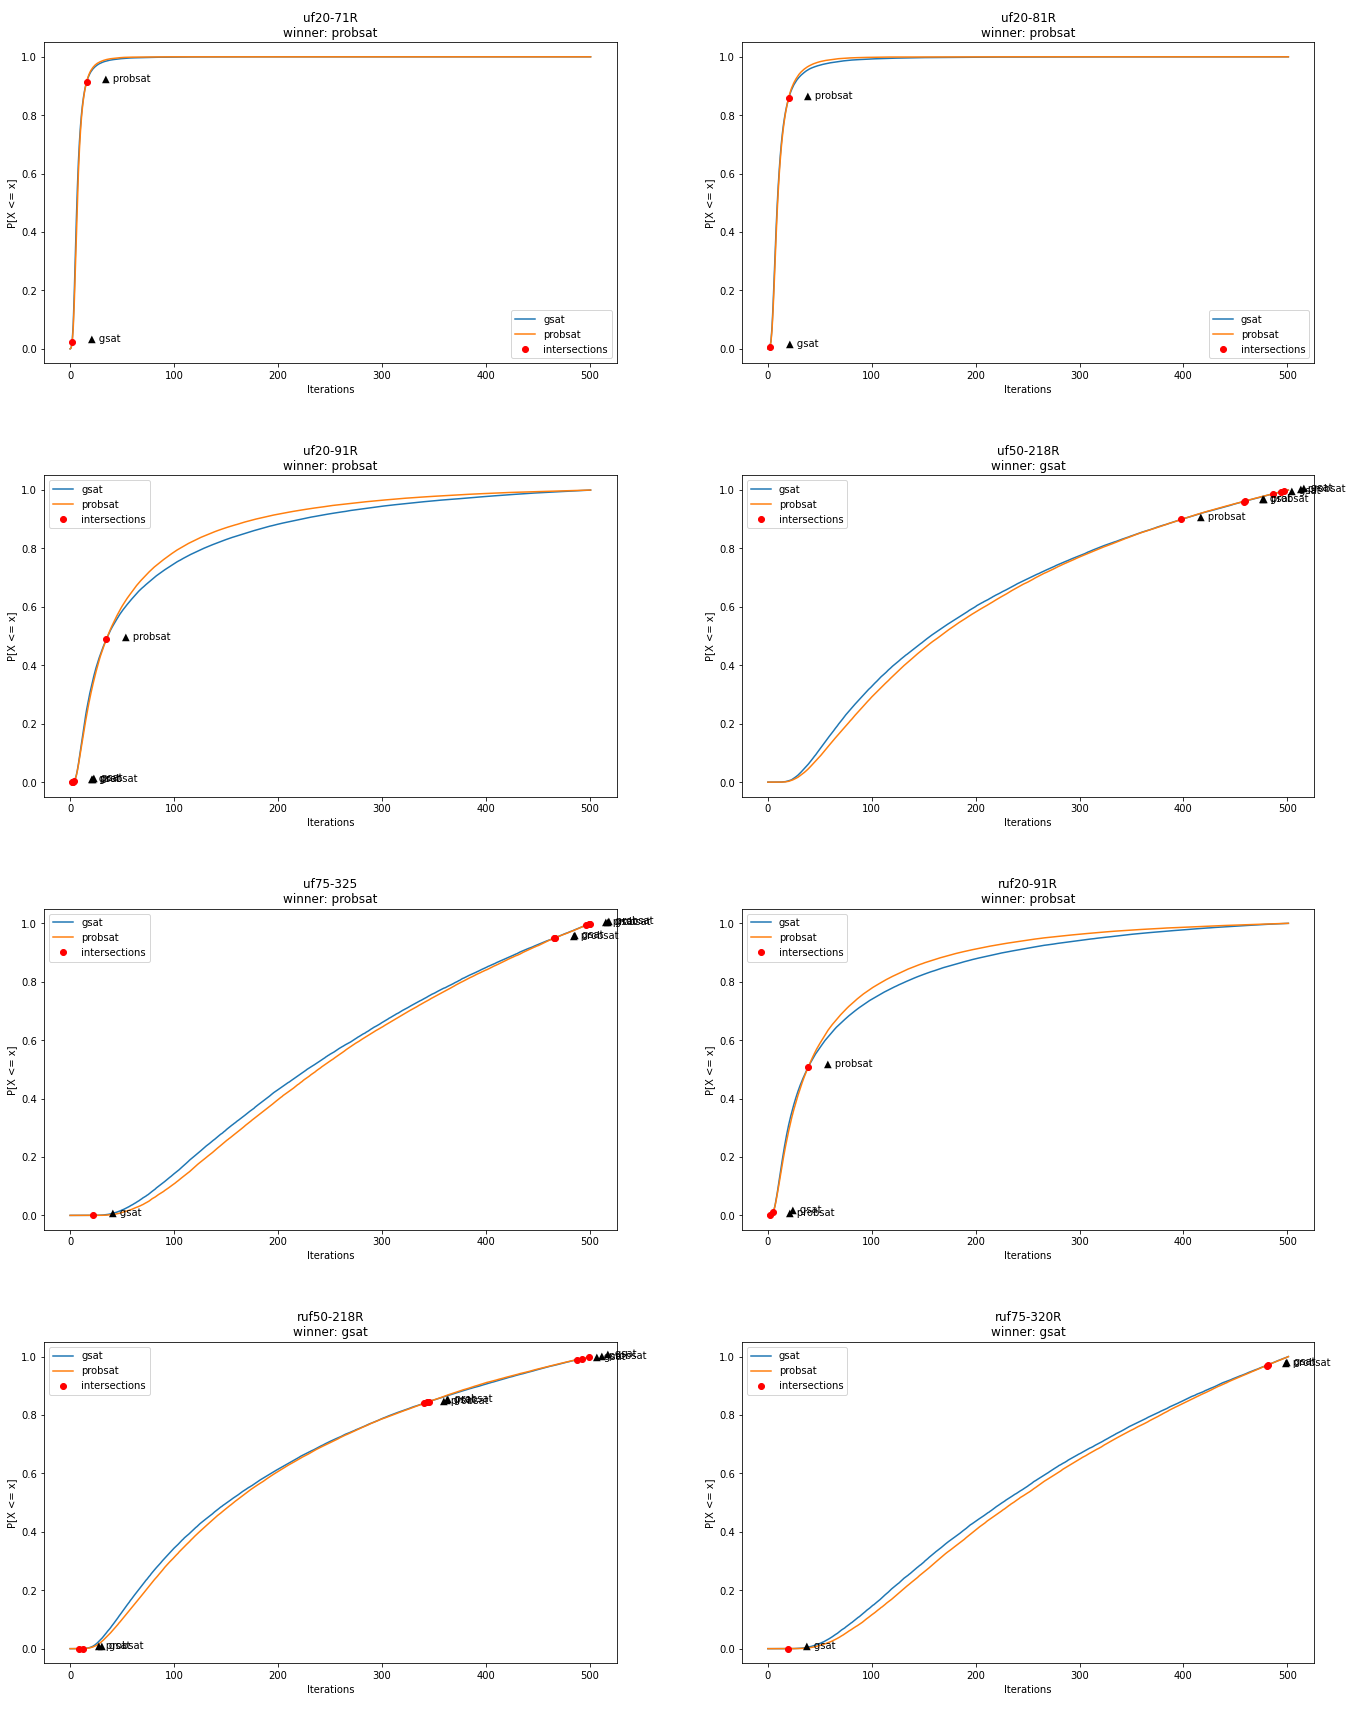
\includegraphics[width=\textwidth]{images/gsat_probsat_success_cdf-1}
        \caption{CDF pro úspěšné běhy algoritmů}
        \label{fig:cdf1}
    \end{figure*}

    \begin{figure*}[h]
        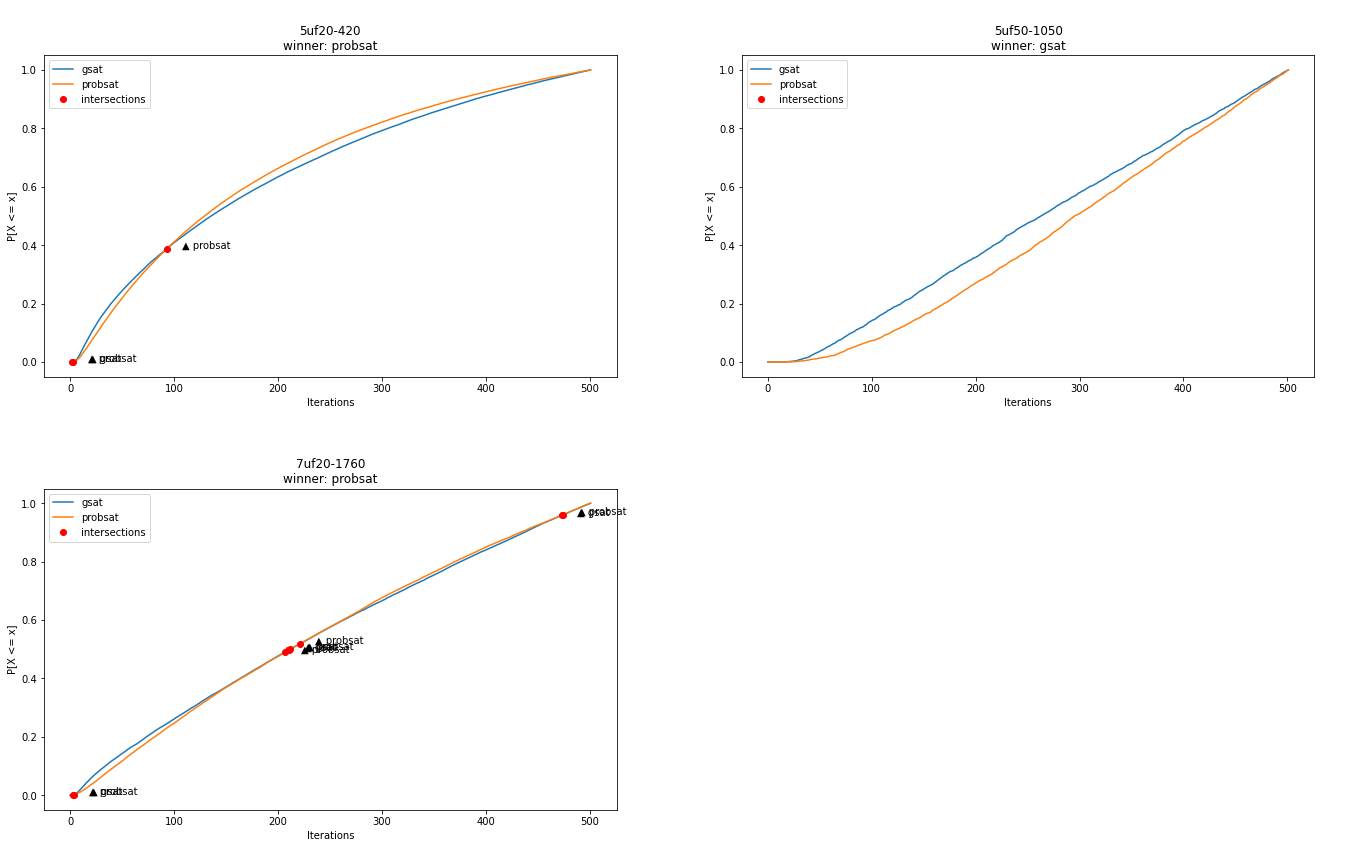
\includegraphics[width=\textwidth]{images/gsat_probsat_success_cdf-2}
        \caption{CDF pro úspěšné běhy algoritmů}
        \label{fig:cdf2}
    \end{figure*}

    Korigovaná distribuční funkce je přenásobená distribuční funkce prametrem $\rho$.
    Parametr $\rho$ je dynamicky počítán pro každou sadu instancí a reprezentuje podíl počtu úspěšných běhů k počtu všech spuštěných běhů.
    Korigovaná distribuční funkce již není distribuční funkcí nějakého statistického rozložení, ale i přesto může sloužit jako
    dobrý indikátor pro porovnání algoritmů.
    Například lze také sledovat trend dominance, křížení funkcí a porovnání absolutního vítěze na dané datové sadě.

    Algoritmus probSAT zvítězil ve všech datových sadách.
    Algoritmus gSAT nezvítězil v žádné datové sadě.

    Tento výsledek dobře koreluje s předchozím výsledkem o úspešnosti algoritmů, kde probSAT měl větší úspěšnost než gSAT.

    \begin{figure*}[h]
        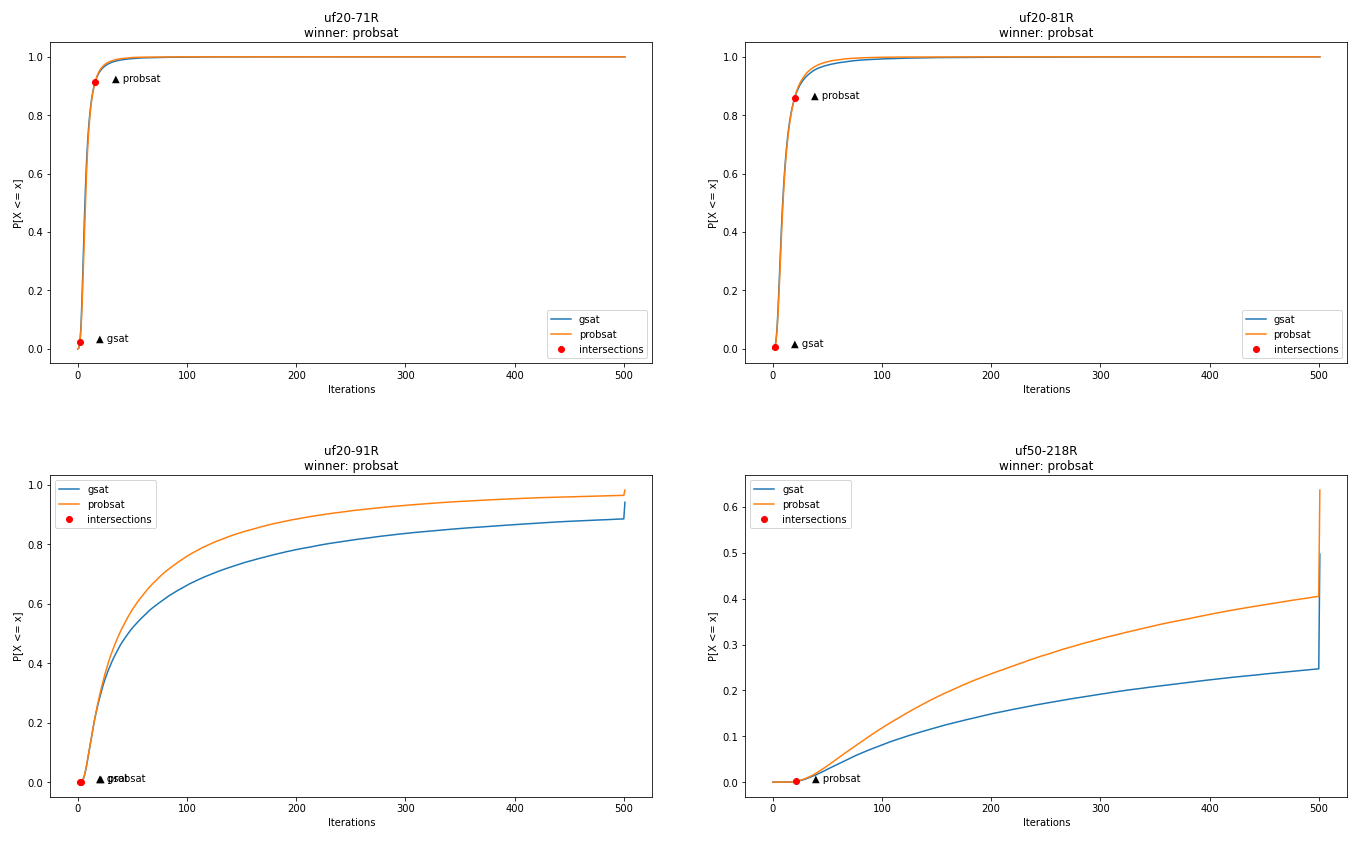
\includegraphics[width=\textwidth]{images/gsat_probsat_revcdf-1}
        \caption{Korigovaná CDF pro běhy algoritmů}
        \label{fig:revcdf1}
    \end{figure*}

    \begin{figure*}[h]
        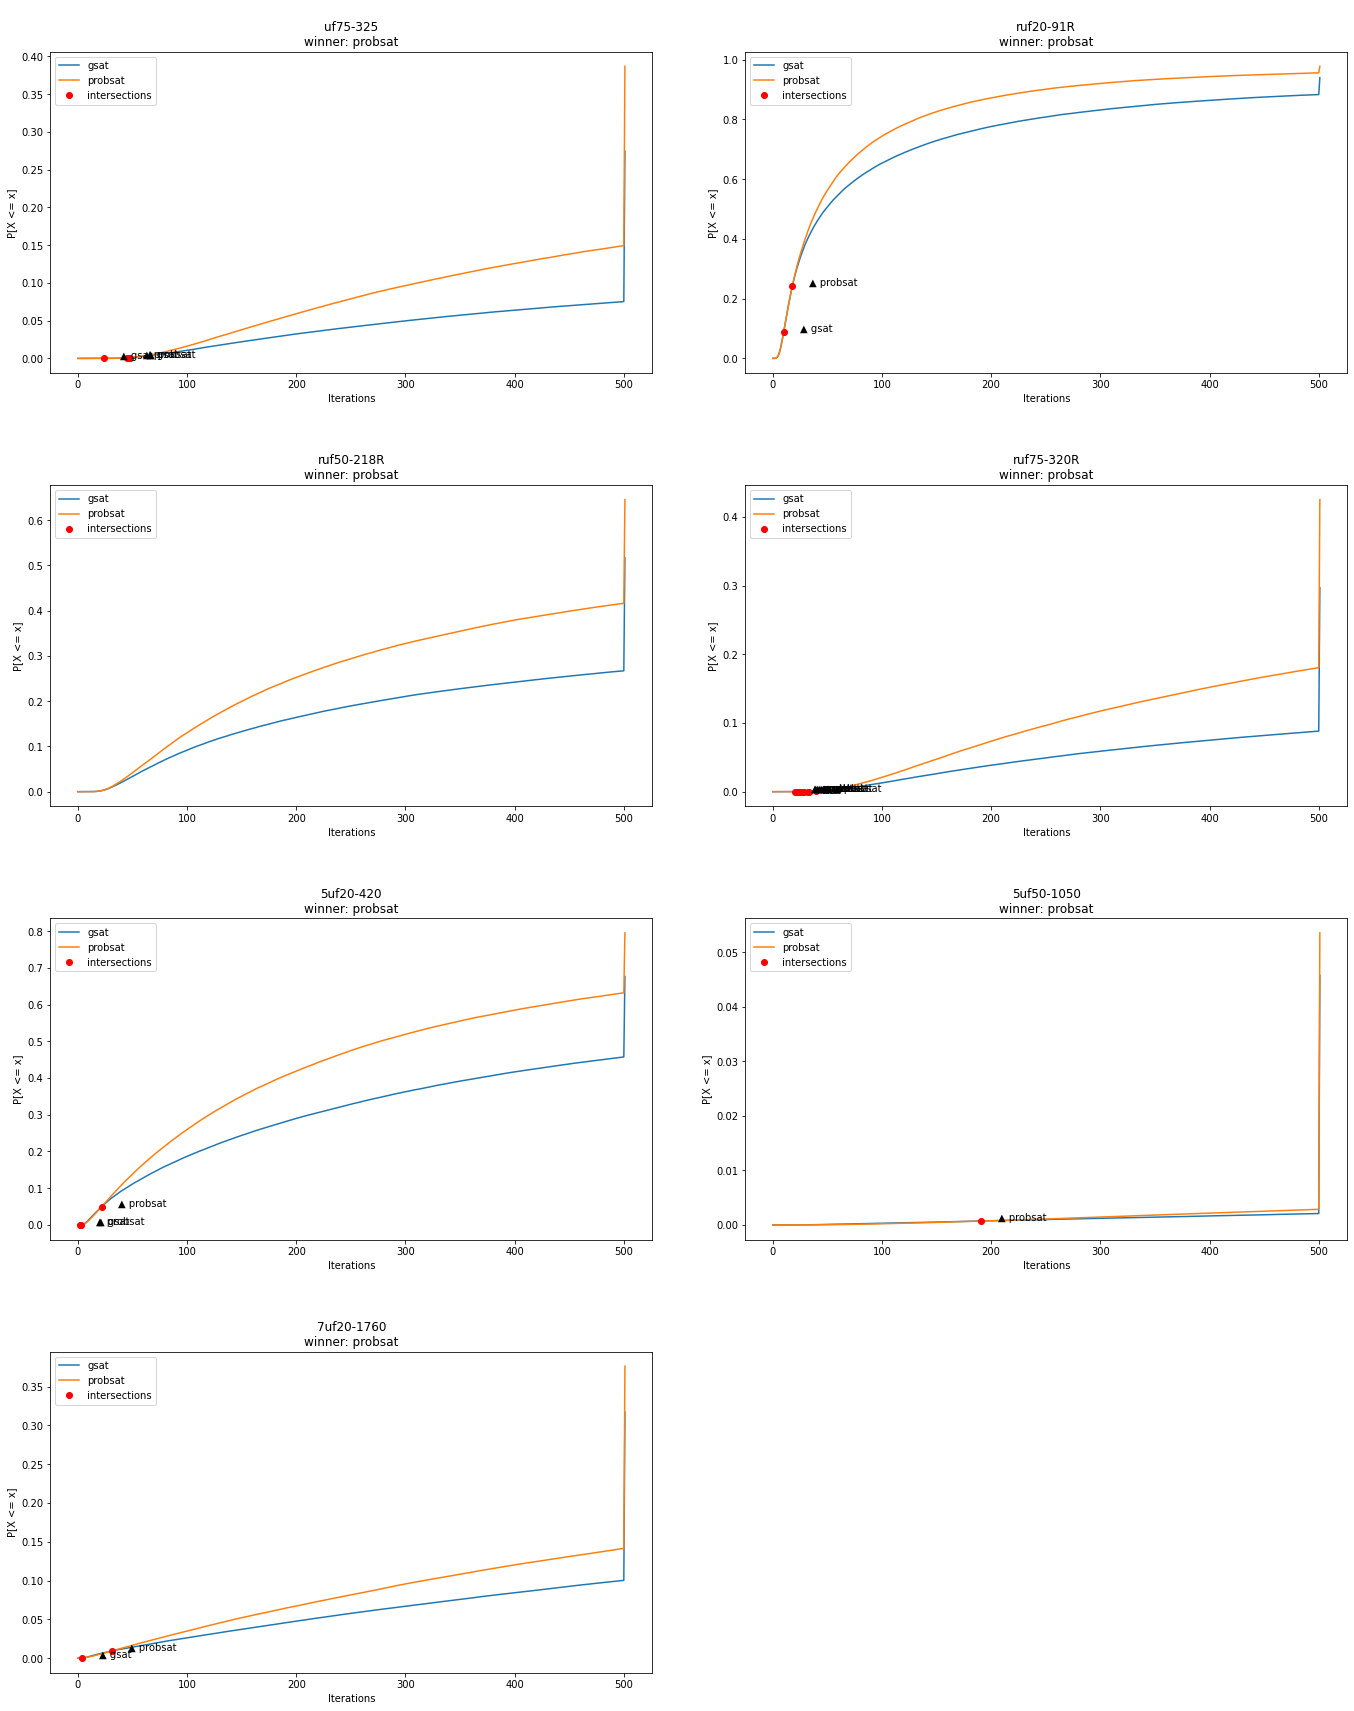
\includegraphics[width=\textwidth]{images/gsat_probsat_revcdf-2}
        \caption{Korigovaná CDF pro běhy algoritmů}
        \label{fig:revcdf2}
    \end{figure*}

    Obrázky~\ref{fig:lognormal1}~a~\ref{fig:lognormal2} zobrazují hustotu pravděpodobnosti počtu iterací v úspešných bězích
    obou algoritmů a pomocí aproximace parametrů lognormalního rozložení také zobrazuje hustotu tohoto rozložení s danými parametry.

    Zde je viditelné, že výsledné počty iterací lze na daných datových sadých považovat za lognormálně rozdělené.

    \begin{figure*}[h]
        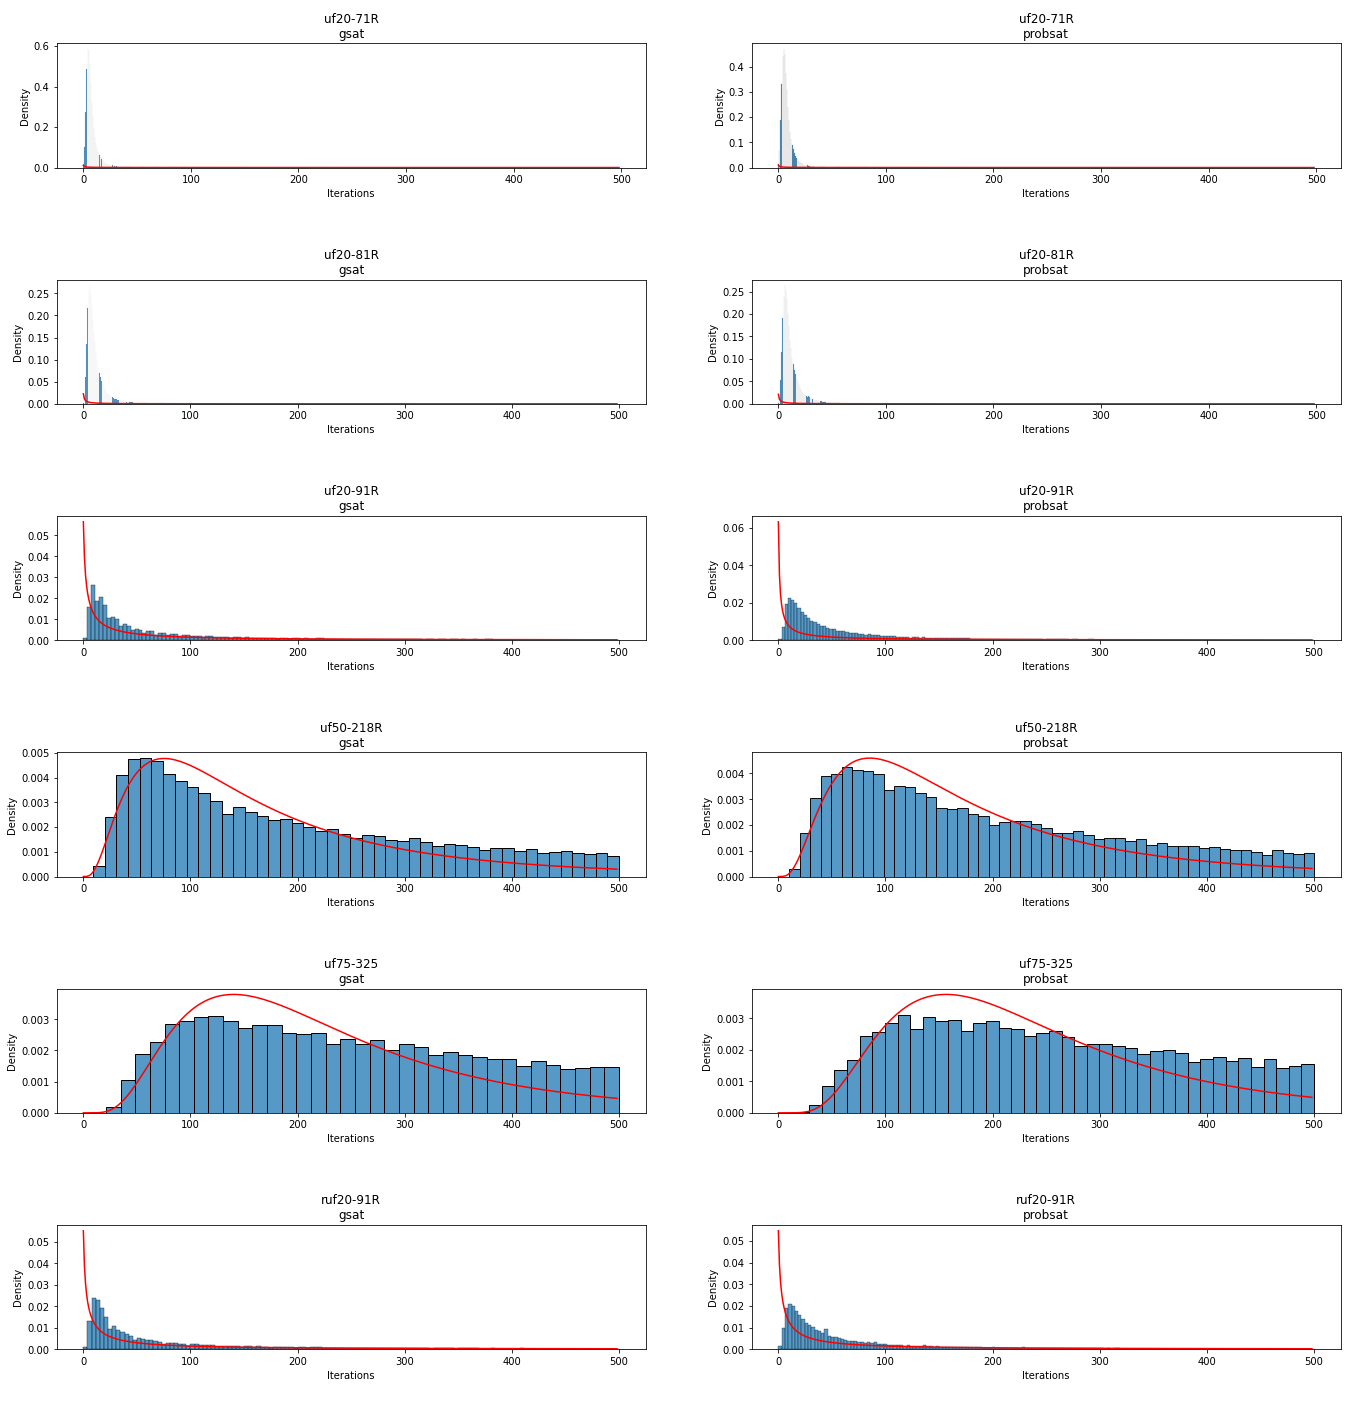
\includegraphics[width=\textwidth]{images/gsat_probsat_pdf_lognormal-1}
        \caption{Lognormální rozložení a hustota experimentálních dat}
        \label{fig:lognormal1}
    \end{figure*}

    \begin{figure*}[h]
        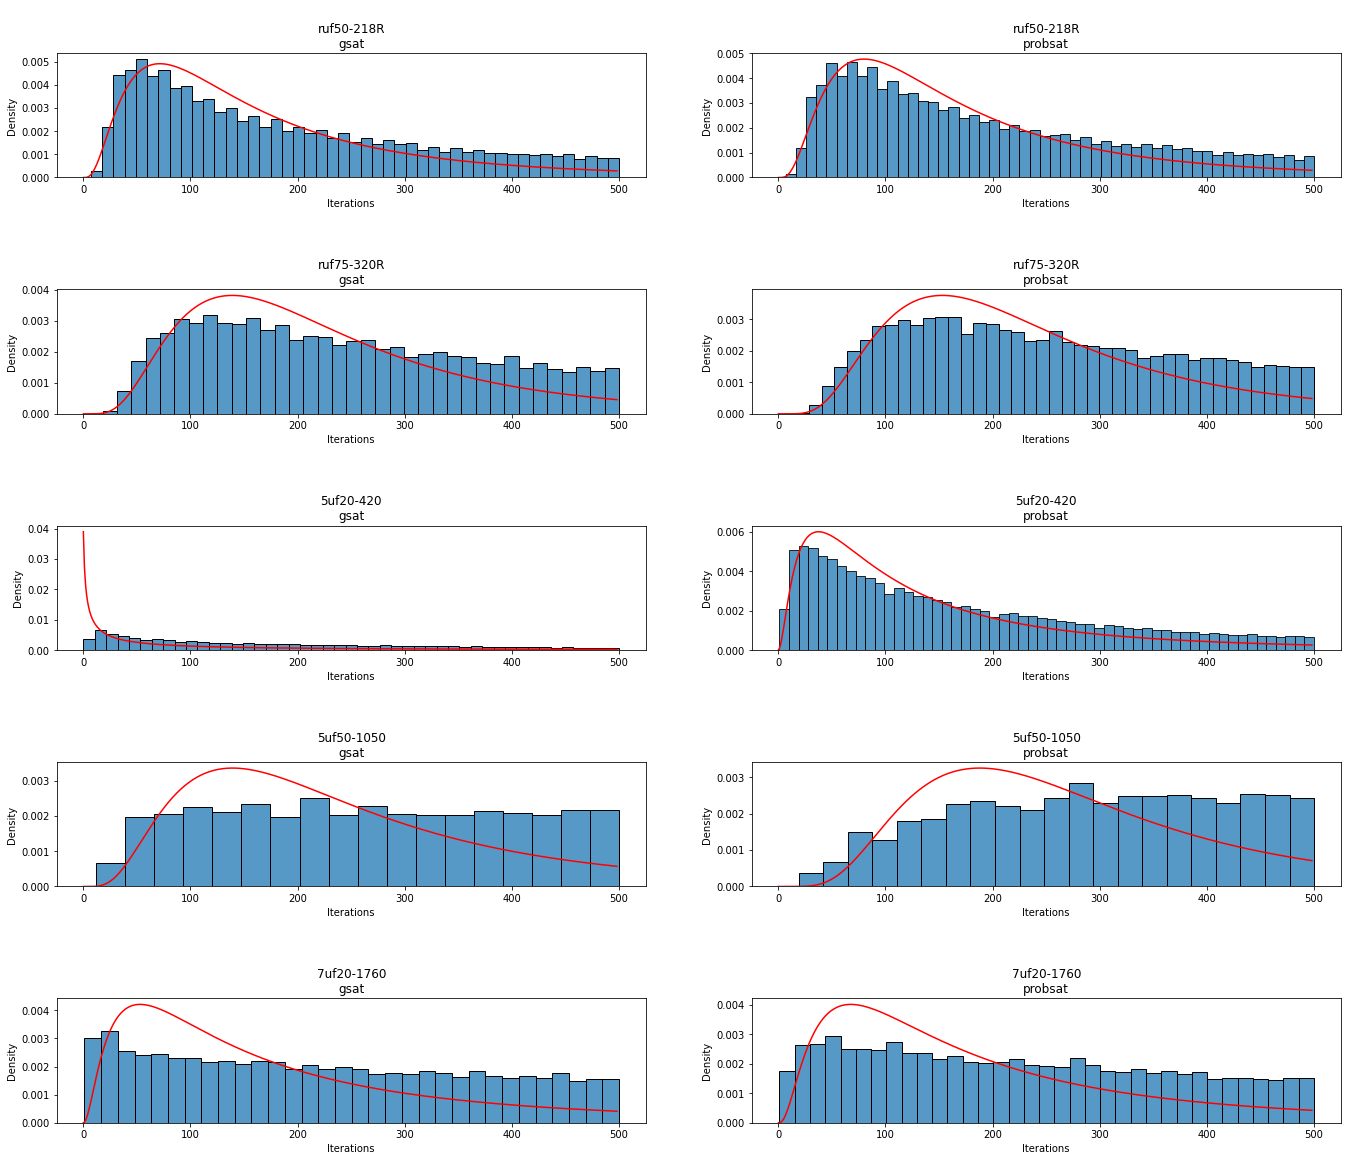
\includegraphics[width=\textwidth]{images/gsat_probsat_pdf_lognormal-2}
        \caption{Lognormální rozložení a hustota experimentálních dat}
        \label{fig:lognormal2}
    \end{figure*}

%------------------------------------------------


    \section{Diskuze}

    Na velkém výběru datových sad byly experimentálně porovnány dva algoritmy (gSAT a probSAT), které oba velmi dobře
    hledají splnitelné ohocnocení SAT formule.
    Z~výsledků experimentu vyšlo, že probSAT má větší procentuální úspěšnost nalezení splňujícího ohodnocení se stejným limitem iterací jako gSAT\@.
    Také bylo pozorováno, že probSAT měl větší pravděpodobnost nalezení splňujícího řešení v daném počtu iterací.

    Pro zajištění lepších výsldků a detailnějšího porovnání je možné použít další (větší) datové sady.
    
    V průběhu tvorby experimentu vznikl nástroj na paralelní spouštění velkého množstí datových sat pro programy gSAT a probSAT,
    který je možné nalézt na adrese \href{https://github.com/zapotocnylubos/ni-kop-compare}{github.com/zapotocnylubos/ni-kop-compare}.
    Tento repozitář také obsahuje Python Notebook, který byl použit pro analýzu výsledků experimentu a generovaní grafů.


%----------------------------------------------------------------------------------------
%	REFERENCE LIST
%----------------------------------------------------------------------------------------

    \clearpage

    \bibliography{literature}
    \bibliographystyle{plain}

%\begin{thebibliography}{99} % Bibliography - this is intentionally simple in this template
%
%\bibitem[Figueredo and Wolf, 2009]{Figueredo:2009dg}
%Figueredo, A.~J. and Wolf, P. S.~A. (2009).
%\newblock Assortative pairing and life history strategy - a cross-cultural
%  study.
%\newblock {\em Human Nature}, 20:317--330.
%
%\end{thebibliography}

%----------------------------------------------------------------------------------------

\end{document}
